\documentclass{article}

\usepackage{aistats2021_author_response}

\usepackage[utf8]{inputenc} % allow utf-8 input
\usepackage[T1]{fontenc}    % use 8-bit T1 fonts
\usepackage{hyperref}       % hyperlinks
\usepackage{url}            % simple URL typesetting
\usepackage{booktabs}       % professional-quality tables
\usepackage{amsfonts}       % blackboard math symbols
\usepackage{nicefrac}       % compact symbols for 1/2, etc.
\usepackage{microtype}      % microtypography
\usepackage{xcolor}         % define colors in text
\usepackage{xspace}         % fix spacing around commands
\usepackage{macro_math}
\usepackage{macro_fan}

\begin{document}

	We thank all the reviewers for providing detailed comments, which we will address in the next version of the paper.
	In this response, we first clarify several high-level questions and then respond to each reviewer's comments.

	\textbf{Clarifying the setting of Section 3.} Both R2 and R3 pointed out that our covariate shift analysis only applies to two tasks where the shared matrix $B$'s rank is $1$.
	While this setting is a special case of a two-layer linear neural net, it corresponds to the important setting of transfer learning (specifically solving $f(B) = ||X^{(1)} B - Y^{(1)}||^2 + ||X^{(2)} B - Y^{(2)}||^2$).
	The transfer learning problem with two tasks is well-motivated from a practical perspective.
	Our result provides precise asymptotics under covariate shift.
	We think it is an excellent research question to study the multiple task setting under covariate shift.
	Several recent works have made progress in the multiple linear regression setting, including (Li et al. (2020)), (Chen et al. (2020) arXiv:2009.11282), (Kong et al. (2020) arXiv:2002.08936).
	However, they all assume that the feature vectors are drawn from an isotropic Gaussian distribution.
	Therefore, while our analysis only applies to two tasks, we believe our work has contributed to studying covariate shift.



	\begin{wrapfigure}{R}{4.75cm}
			\vspace{-0.2in}
		\caption{Improved result.}\label{fig_update}
		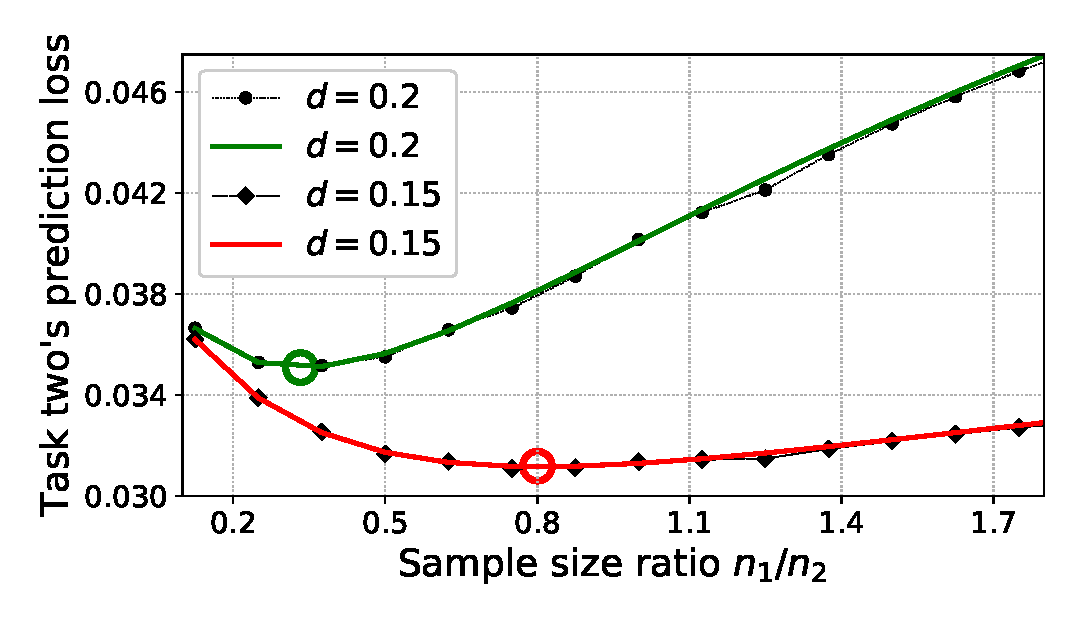
\includegraphics[width=4.75cm]{sample_ratio_several_d.eps}
		\vspace{-0.4in}
	\end{wrapfigure}
	%------------------------------------------
%	{\lipsum[2-3]
%		\par
%	Figure~\ref{wrap-fig:1} is a wrapped figure.


\textbf{The gap between the theory and experiment in Fig 2.b?} Thanks to R2 and R3 for pointing out this gap.
	We have improved our result so that the theory matches experiment in Fig 2.b (see Figure \ref{fig_update} for the updated result).
	To derive the new results, we use the identity $\tr\left[(X_1^\top X_1 + X_2^\top X_2)^{-2}(X_1^\top X_1)^2\right]= \left.\frac{\rm{d}}{{\rm d} t}\right|_{t=0} \tr\left[(X_1^\top X_1 + t(X_1^\top X_1)^2 + X_2^\top X_2)^{-1}\right]$. To calculate the trace of the inverse of $X_1^\top X_1 + t(X_1^\top X_1)^2 + X_2^\top X_2$, we need to study its asymptotic eigenvalue distribution for $t$ close to 0. This can be done by the same technique in our paper.  %DESCRIBE THE IDEA.

	\textbf{Can any of the results in Section 3 be obtained from a straightforward application of a generalized MP theorem?}
	Thanks for raising this question. R2 is correct that the variance equation in Corollary 3.3 can be obtained from the MP law.
	However, to the best of our knowledge, the bias equation in Corollary 3.3 and Example 3.4 cannot be obtained from the MP law.
	Regarding the paper Ledoit and P{\'e}ch{\'e} (2011) mentioned by R2, the authors deal with a single sample covariance matrix $X^\top X$, where the row vectors of $X$ have the same population covariance matrix.
	This setting does not apply to two sample covariance matrices $X_1^\top X_1$ and $X_2^\top X_2$ with different population covariance matrices.
	In particular, if we stack the rows of $X_1$ and $X_2$ into one random matrix $X$, then the row vectors of $X$ have different covariance matrices.
	As R2 asked about, our method also provides a better convergence rate than the method of Ledoit and P{\'e}ch{\'e} (2011).
	%Moreover, the convergence rate using the method of Ledoit and P{\'e}ch{\'e} (2011) is worse than .

	\textbf{Response to R1.} Please see our response to the detailed comments.
	\textbf{(8-i)} Yes, the variance decreases because $||{a_i^{\star}}||^2 \le 1$.
	The bias increases because the bias of single-task learning (the ordinary least squares solution) is zero when $n > p$.
	\textbf{(8-ii)} By lower order terms, we mean any term that vanishes to zero when $p$ increases to infinity.
	\textbf{(8-iii)} The sum of $||{a_i^{\star}}||^2$ is one because $A^{\star}$ is a rank-$1$ projection matrix.
	\textbf{(8-iv)} %We want to point out that the problem setting in Section 3 is in general non-convex. Therefore, it is not possible to explicitly solve $A_1, A_2$ without making further assumptions.
	We can assume knowledge of $A_1 \in \mathbb R, A_2 \in \mathbb R$ without loss of generality by solving them numerically using a subset of training data points (e.g. $\sqrt{p}$ suffices).
	The sampling error of the numerical solution is $O(\exp(-p))$.

	\textbf{Response to R2.} We thank the reviewer for providing detailed feedback.
	Response to questions under Section 8.
	\textbf{(i)}
	In the over-parametrized regime, the minimum solution of $f(A ,B)$ (equation 1) reduces to single-task learning  (cf. Proposition 1 in Wu et al., 2020).
	Hence, studying this regime is problematic without adding explicit regularization or implicit algorithmic biases.
	These are interesting research questions but beyond the scope of our work.

	Response to questions under Section 3.
	\textbf{(1-ii)} We would like to clarify that the purpose of the examples is to explain empirical phenomena of multi-task and transfer learning related to sample size ratios and covariate shifts.
	We believe that our examples have provided important initial insights toward understanding the effect of varying sample size ratios and covariate shifts.
	See Appendix A for evaluation in a real-world data setting.
%	We will address these issues and the other clarification questions in the next version of the paper.

	\textbf{Response to R3.}
	We thank the reviewer for the favorable review.
	Regarding the question of how the prediction loss varies with $r$, our result implies the following corollary of Theorem 2.1.
	Suppose that the singular values of ${B^{\star}}^{\top}\Sigma B^{\star}$ are $\lambda_1, \lambda_2, \dots, \lambda_t$ in decreasing order.
	If we increase $r$ by $1$, the bias reduces by $\lambda_{r+1}$ while the variance increases depending on the singular vector of  ${B^{\star}}^{\top}\Sigma B^{\star}$ corresponding to $\lambda_{r+1}$.
	As an example of this corollary, we can show that in the setting of Example 2.2, the average prediction loss of all tasks is minimized when $r$ is one.
	We also thank the reviewer for suggesting the related work.
	We will add these related works to the next version of the paper.

	\textbf{Response to R5.}
	In response to the reviewer's comments, we explain the high-level purpose of our work and the importance of why one should care about analyzing the sample size ratios.
	Hard parameter sharing is a widely used empirical approach to performing multi-task learning.
	However, there remain significant challenges for applying hard parameter sharing in practice.
%	The first challenge is negative transfer, which occurs when the performance of MTL is worse than STL.
	Dealing with unbalanced datasets is one such challenge (He et al. (2020) arXiv:2001.06782).
	Vu et al. (2020 arXiv:2005.00770) conducted a large-scale evaluation and observed that sample sizes critically affect the performance of transfer learning.
	Our result rigorously analyzes the effect of varying sample size ratios using bias-variance tradeoffs and imply a practically useful progressive training algorithm (cf. Appendix A).
\end{document}
